\newpage 
\section{Introduction}
\subsection{Cas pratique}
Dans ce travail pratique, nous devons créer une application permettant de gérer une To Do List. Deux vues seront créées. L'application pourra naviguer entre les deux.\\
Dans la première vue, on retrouve une représentation des tâches
existantes. Chaque entrée est constituée d’une image (« ! » ou vide ) ainsi que d’un descriptif de
la tâche.\\
L'autre vue permet l’ajout d’une nouvelle tâche dans la liste. Un bouton sert à indiquer si la tâche est urgente ou non, un champ de text permet de recevoir le nom de la tâche.\\
L'image ci-dessous présente la solution de design proposée par la donnée.
\begin{figure}[H]
	\begin{center}
		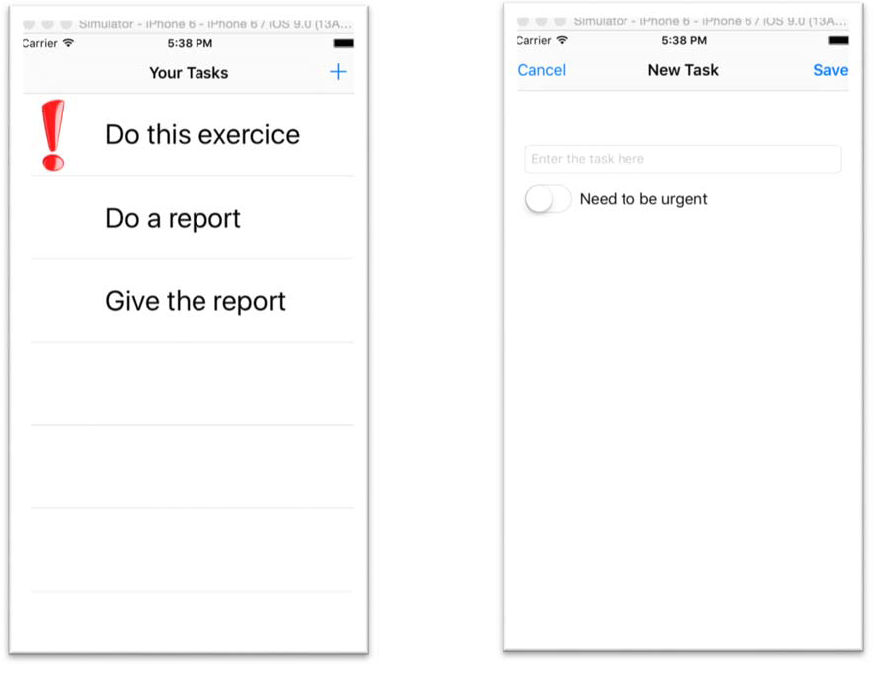
\includegraphics[width=10cm]{img/intro.png}
		\caption{Vues de l'application}
		\label{intro}
	\end{center}
\end{figure}

\subsection{Buts}
\begin{enumerate}
	\item Se familiariser avec le langage swift
	\item Utilisation de "Navigation Controller"
	\item Comprendre le développement et déploiement d'application iOS.
\end{enumerate}

\subsection{Objectifs}
\begin{enumerate}
	\item Création de la vue pour l’ajout d’une tâche
	\item Connecter la vue avec le "view controller" pour l’ajout et implémenter le contrôleur.
	\item Création du modèle qui représente une tâche
	\item Création de la vue pour lister les tâches
	\item Connecter la vue avec le "table view controller" pour la gestion de la table et implémenter le contrôleur
	\item  Mise en place de la navigation
\end{enumerate}